\section{Linear Regression}

The linear regression analysis consists of statistical analysis to verify the existence of a functional relationship between a dependent variable with one or more independent variables. In other words, this analysis consists of obtaining a linear equation that tries to explain the variation from the dependent variable by variation from the independent variable level.

The statistical model for this case should be:
\begin{equation} 
    \label{eqn_example}
    y = a.x + b
\end{equation}

Where $y$ represents the dependent variable, $a$ represents the line slope of the linear model, and $b$ represents the y-axis intercept. The regression line is a method to calculate the parameters $a$ and $b$.

The determination coefficient, frequently called $R^2$, or simply $r^2$, for the linear regression case, provide auxiliary information to the analysis of the result of regression variance, as a way to verify if the proposed model is suitable or not to describe the phenomenon.

In this work, we verified how close is the relationship between the \textit{probability of failure} independent variable and the other dependent variables: \%LSS and \%UEQ to a linear equation.

To discover an equation that represents the studied phenomenon, we could build a graph, called \textit{Scatter Plot}, to verify by visualization how is the variation between the dependent and independent variables.

To discover an equation that represents the studied phenomenon, we could build a graph, called scatter plot, to verify by visualization how is the variation between the dependent and independent variables. Figures \ref{fig-linear-regression-scatter-plots-lss} and \ref{fig-linear-regression-scatter-plots-ueq} are the scatter plots for \%LSS and \%UEQ for each algorithm, respectively. In these figures, we can see the line from the linear equation from the estimated model that used the minimum mean square error as criteria. The red dotted line represents the bounds for 95\% of the confidence interval.

\begin{figure}[H]
    \centering
     \begin{subfigure}{.5\textwidth}
     \centering
     \frame{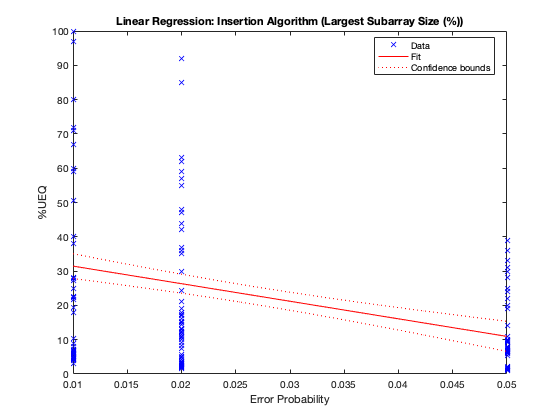
\includegraphics[scale=0.45]{figures/linear_regression_scatter_plot_lss_bubble.png}}
     \textsf{\caption[Bubblesort algorithm.]{Bubblesort algorithm.\label{fig-linear-regression-scatter-plot-lss-bubble}}}
     \end{subfigure}%
     \begin{subfigure}{.5\textwidth}
     \centering
     \frame{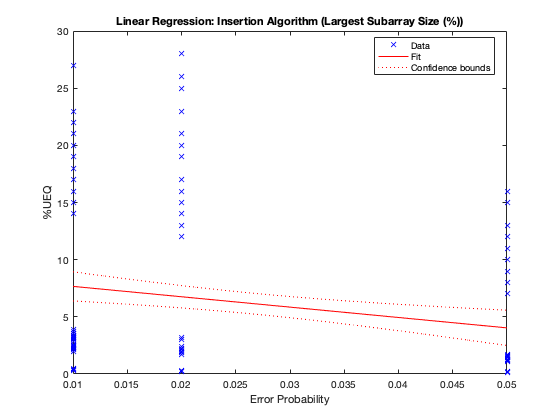
\includegraphics[scale=0.45]{figures/linear_regression_scatter_plot_lss_insertion.png}}
     \textsf{\caption[Insertionsort algorithm.]{Insertionsort algorithm.\label{fig-linear-regression-scatter-plot-lss-insertion}}}
     \end{subfigure}
     \begin{subfigure}{.5\textwidth}
     \centering
     \frame{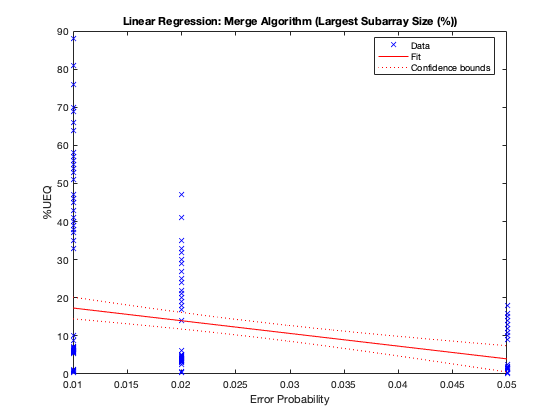
\includegraphics[scale=0.45]{figures/linear_regression_scatter_plot_lss_merge.png}}
     \textsf{\caption[Mergesort algorithm.]{Mergesort algorithm.\label{fig-linear-regression-scatter-plot-lss-merge}}}
     \end{subfigure}%
     \begin{subfigure}{.5\textwidth}
     \centering
     \frame{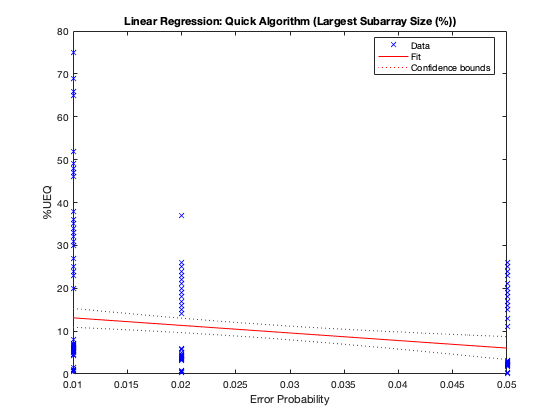
\includegraphics[scale=0.45]{figures/linear_regression_scatter_plot_lss_quick.png}}
     \textsf{\caption[Quicksort algorithm.]{Quicksort algorithm.\label{fig-linear-regression-scatter-plot-lss-quick}}}
     \end{subfigure}
     \caption{Scatter plot and the linear regression for \%LSS versus Probability of Failure.}
    \label{fig-linear-regression-scatter-plots-lss}
  \end{figure}

  \begin{figure}[H]
    \centering
     \begin{subfigure}{.5\textwidth}
     \centering
     \frame{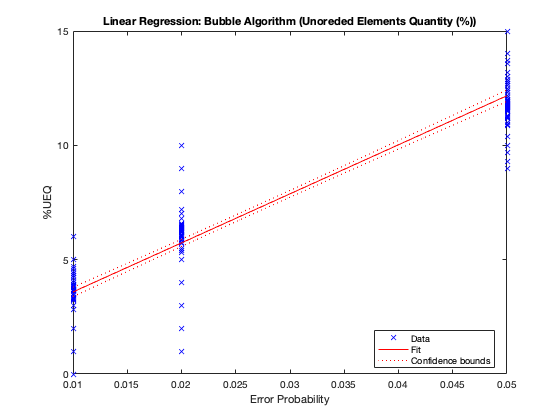
\includegraphics[scale=0.45]{figures/linear_regression_scatter_plot_ueq_bubble.png}}
     \textsf{\caption[Bubblesort algorithm.]{Bubblesort algorithm.\label{fig-linear-regression-scatter-plot-ueq-bubble}}}
     \end{subfigure}%
     \begin{subfigure}{.5\textwidth}
     \centering
     \frame{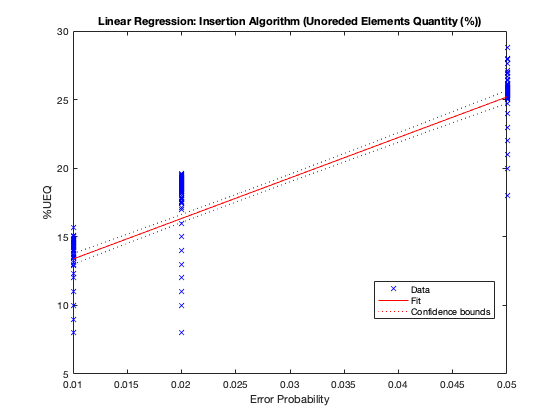
\includegraphics[scale=0.45]{figures/linear_regression_scatter_plot_ueq_insertion.png}}
     \textsf{\caption[Insertionsort algorithm.]{Insertionsort algorithm.\label{fig-linear-regression-scatter-plot-ueq-insertion}}}
     \end{subfigure}
     \begin{subfigure}{.5\textwidth}
     \centering
     \frame{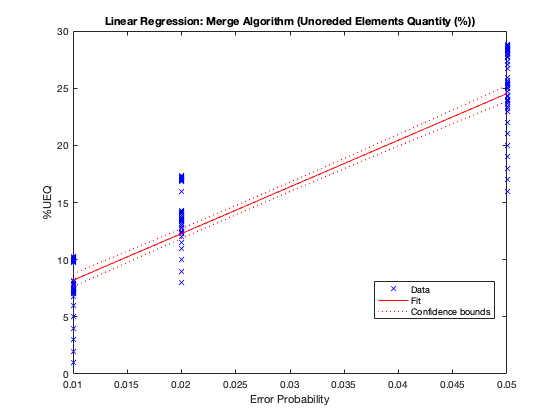
\includegraphics[scale=0.45]{figures/linear_regression_scatter_plot_ueq_merge.png}}
     \textsf{\caption[Mergesort algorithm.]{Mergesort algorithm.\label{fig-linear-regression-scatter-plot-ueq-merge}}}
     \end{subfigure}%
     \begin{subfigure}{.5\textwidth}
     \centering
     \frame{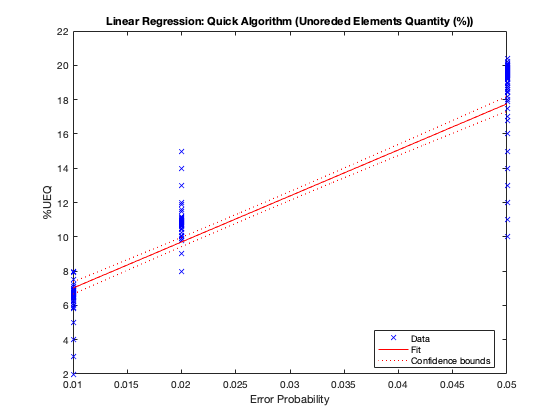
\includegraphics[scale=0.45]{figures/linear_regression_scatter_plot_ueq_quick.png}}
     \textsf{\caption[Quicksort algorithm.]{Quicksort algorithm.\label{fig-linear-regression-scatter-plot-ueq-quick}}}
     \end{subfigure}
     \caption{Scatter plot and the linear regression for \%UEQ versus Probability of Failure.}
    \label{fig-linear-regression-scatter-plots-ueq}
  \end{figure}

  However, we can verify that the points at scatter plots, don't have perfect adjust to the proposed math model line. There are, in major part, a great distance between the points at the plot and the model line. This distance happens because, in each probability of failure, we have many values of the dependent variable and with large dispersion. This situation explains why the determination coefficient $r^2$ has a low value in most of the cases.

  The Tables \ref{table-linear-regression-lss} and \ref{table-linear-regression-ueq} below shows the parameters for linear regression of both variables \%LSS and \%UEQ. For \%UEQ variable, we found better (from 0.809 to 0.899) $r^2$ than \%LSS (from 0.0499 to 0.141) variable for all algorithms.

  \begin{table}[H]
    \caption{Parameters from linear regression for the \%LSS variable.}
    \begin{center}
    \begin{tabular}{|c|c|c|c|c|}
    \hline
    \textbf{Parameter} & \textbf{Bubblesort} & \textbf{Quicksort} & \textbf{Mergesort} & \textbf{Insertionsort} \\
    \hline
    Intercept (b) & 36.576 & 14.86 & 20.651 & 8.5707 \\
    \hline
    Slope (a) & -512.32 & -176.4 & -333.64 & -90.711 \\
    \hline
    $r^2$ & 0.141 & 0.0499 & 0.101 & 0.0399 \\
    \hline
    Root Mean Squared Error (RMSE) & 21.5 & 13.1 & 17 & 7.59 \\
    \hline
    \end{tabular}
    \label{table-linear-regression-lss}
    \end{center}
\end{table}

\begin{table}[H]
    \caption{Parameters from linear regression for the \%UEQ variable.}
    \begin{center}
    \begin{tabular}{|c|c|c|c|c|}
    \hline
    \textbf{Parameter} & \textbf{Bubblesort} & \textbf{Quicksort} & \textbf{Mergesort} & \textbf{Insertionsort} \\
    \hline
    Intercept (b) & 1.4429 & 4.3258 & 4.1165 & 10.426 \\
    \hline
    Slope (a) & -214.56 & 268.59 & 408.4 & 295.39 \\
    \hline
    $r^2$ & 0.899 & 0.823 & 0.809 & 0.826 \\
    \hline
    Root Mean Squared Error (RMSE) & 1.23 & 2.12 & 3.38 & 2.31 \\
    \hline
    \end{tabular}
    \label{table-linear-regression-ueq}
    \end{center}
\end{table}